\chapter{身体運動のばらつきを評価するための最適な実験条件}
4章で述べたボタン押し課題でボタンの押下時間間隔を記録すると,聴覚フィードバックに遅延がない場合でも理想的なボタンの押下間隔にはならずいくらかのばらつきが発生する.これは,遅延聴覚フィードバックが身体運動に与える影響の調査において発生する本質的なばらつきであると考えられる.そのため,聴覚フィードバックに遅延がない場合でのばらつきが小さくなるような実験条件を用いれば,遅延による影響がより顕著に現れることが期待される.そこで,本章ではこの調査における最適な実験条件を明らかにするために,以下の実験から実験条件によるばらつきの変化を調査する.
\begin{enumerate}[leftmargin=*, label=実験(\arabic*)] % ラベルの設定
  \item メトロノームの合図音のBPMを変化させたときのボタンの押下時間間隔のばらつきの変化を調べる.
  \item 分散の計算に用いるデータの個数の違いによるばらつきの変化を調べる.
\end{enumerate}
実験(1)と実験(2)では,聴覚フィードバックの遅延時間を一般的に影響のない遅延時間とされている10[ms]に設定する.
\section{ボタンを押下する間隔の最適な条件}
この実験では,1分間にボタンを押下する回数を70回から110回までの5種類に変化させる.20代の被験者8人を対象に調査を行った.図\ref{fig:bpm}にボタンを押下する間隔と評価指標の関係を示す.この図から1分間に80回の間隔でボタンを押下するときが最も標準偏差が小さいことがわかる.このため,これ以降の実験では,ボタンを押下する時間間隔を1分間に80回とする.
\begin{figure}[b]
  \centering
  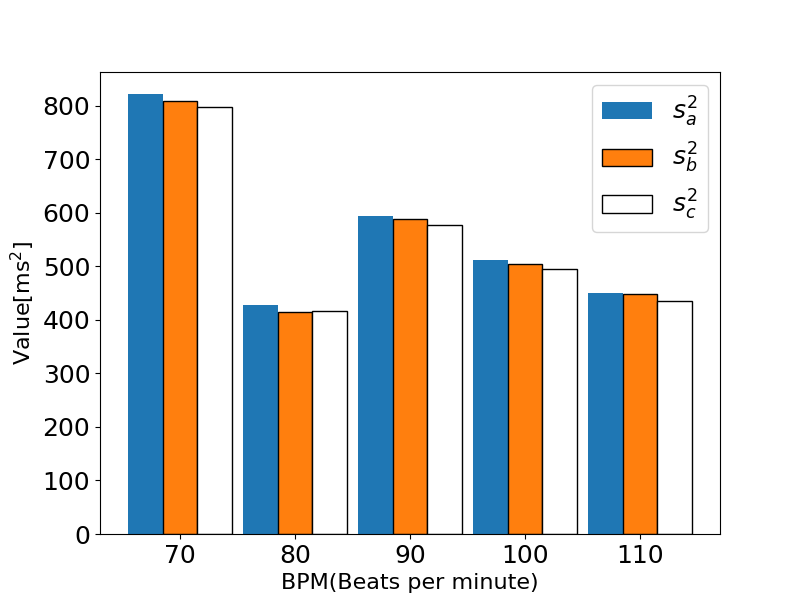
\includegraphics[scale=0.6]{figures/Yobi/BPM_Change.png}
  \caption{ボタンを押下する間隔と評価指標の関係}
  \label{fig:bpm}
\end{figure}
\section{ボタンを押下する回数の最適な条件}
本節では,遅延時間を10[ms],kを9に固定する.図\ref{fig:NumberofSamples_Sa_Sc}lを10から30まで1ずつ変化させながら$s^2_{a}$および$s^2_{c}$を算出し,被験者数で平均している.図\ref{fig:Numberofsamples_Sb}では同様に$s^2_{b}$を算出し,被験者数で平均している.これらの図から,評価指標の値の算出に使用するデータの個数が20を超えると,値がデータの個数の増加に伴い,大きくなっていくことがわかる.そのため,実験条件によって発生するばらつきを最小限に抑えるためには分析するデータの個数を20個以下とすればよいと考えられる.以降の実験では,観測値全体のばらつきを評価するときのデータのサイズは,20個とする.
\begin{figure}[bt]
  \centering
  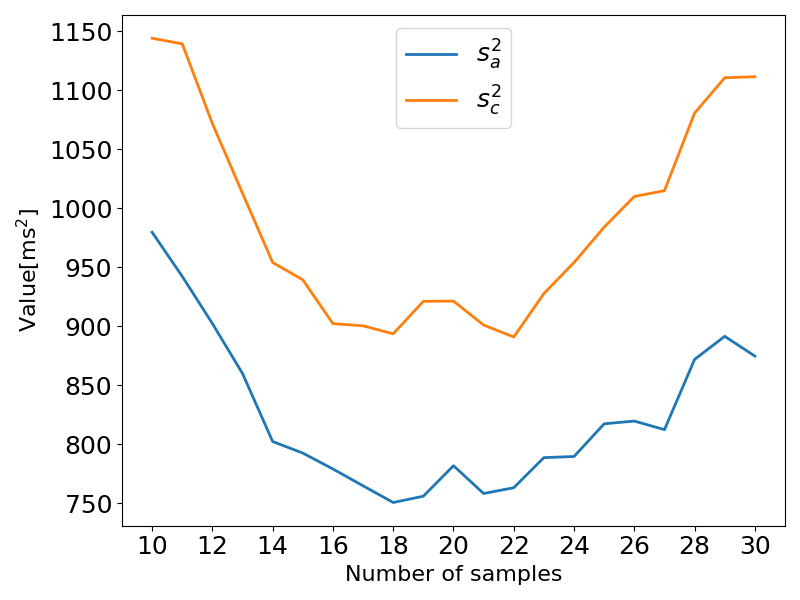
\includegraphics[scale=0.6]{figures/Yobi/NumberOfSamples_s1s3.png}
  \caption{使用するボタンの押下時間間隔のデータ個数と評価指標の関係}
  \label{fig:NumberofSamples_Sa_Sc}
\end{figure}
\begin{figure}[bt]
  \centering
  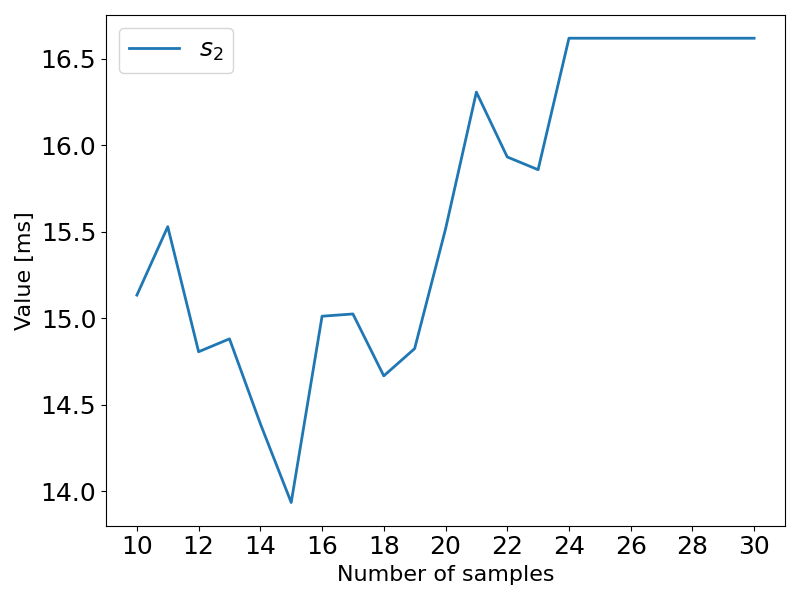
\includegraphics[scale=0.6]{figures/Yobi/NumberOfSamples_median.png}
  \caption{使用するボタンの押下時間間隔のデータ個数と評価指標の関係}
  \label{fig:Numberofsamples_Sb}
\end{figure}

% \section{評価指標の値を算出する上での最適な条件}
% 先行研究[重松さんの論文]では,実験者が指定するボタンの押下回数を20回から10回間隔で40回までの3種類に変化させ,最も評価指標の値が小さくなるようなデータの開始点を算出した.本研究でも同様に評価指標の値が最も小さくなるようなデータの開始点を算出するために遅延を感じないとされている遅延時間10[ms]という条件でボタン押し課題を行い,本質的なばらつきが発生しないような最適な実験条件を探る.この実験では,ボタンの押下回数を40回に指定する.また,遅延時間を10[ms]に固定し行う.被験者は,20代の男女10名である.図6.2,図6.3に評価指標の時間変化を示す.また,図6.3に予備調査で遅延時間を変化させたときの結果の10msの時の結果を示す.被験者は,20人である.
% \newpage
% \begin{figure}[tb]
%   \centering
%   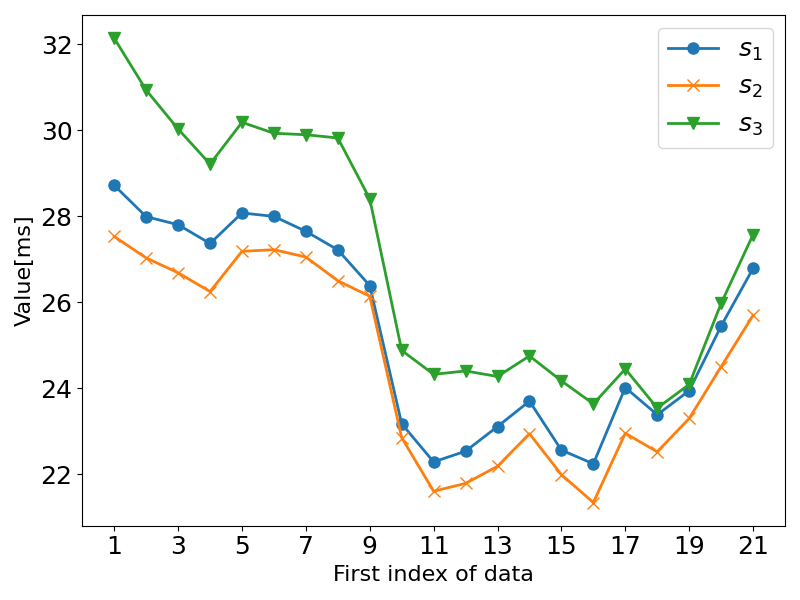
\includegraphics[scale=0.45]{figures/Yobi/Yobi_10ms_TimeChange.png}
%   \caption{評価指標の時間変化}
% \end{figure}
% \begin{figure}[tb]
%   \centering
%   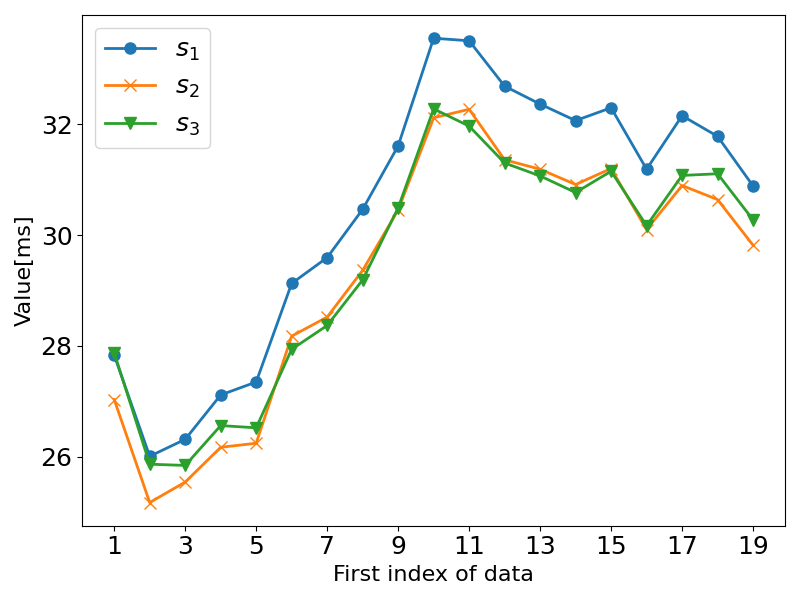
\includegraphics[scale=0.45]{figures/Yobi/Yobi_10ms_tyuuusyutu.png}
%   \caption{評価指標の時間変化}
% \end{figure}
% \newpage
\section{遅延を発生させる最適なタイミング}
本節では,6.1節で規定された適切なボタン押下間隔を用いて,遅延を発生させる最適なタイミングを検証する.実験Aでは,被験者による予備調査後の口頭アンケート結果から,「遅延を感じなかった」あるいは「遅延を感じたが操作感に影響はなかった」との意見が寄せられた.この結果を踏まえ,「ボタン押下時の合図音の遅延が一定であれば,被験者は遅延に適応し,ボタン押下の時間間隔に及ぼす影響が減少する」との仮説を立て,「合図音の遅延が毎回でない場合,慣れの影響が軽減され,遅延聴覚フィードバックの影響が明確に観察される」と考えた.この仮説を検証するために,実験Bでは,ボタンの押下回数が4の倍数に達したときだけ遅延を発生させるシステムを用いて,遅延聴覚フィードバックが身体運動に及ぼす影響を分析した.
 \begin{enumerate}[leftmargin=*, label=実験(\Alph*)]
    \item ボタンを押下したときの合図音が常に遅延する場合
    \item ボタンを押下するときの合図音がボタンの押下回数が4の倍数に達したときのみ遅延する場合
 \end{enumerate}
 
上記2つの実験を行い,聴覚フィードバックの遅延時間とボタンの押下時間隔のばらつきの関係が読み取り可能である実験条件を探る.
\subsection{調査方法}
若年者を対象に行った遅延聴覚フィードバックが身体運動に与える影響の調査方法を以下に示す.実験Aと実験Bともに調査の方法は同様である.
\begin{enumerate}[leftmargin=*]
  \item 被験者に図4.1のシステムを用意する.
  \item 4章の4.1節の手順1から手順2まで述べた方法によって,ボタン押し課題を実施する.
  \item ヘッドホンから出力されるボタン押下の合図音の遅延時間をランダムに変更して実験者が指定した回数だけ手順2を繰り返す.このとき,実験者が提示する回数は,6.2節で提示する遅延時間の種類である.また,遅延時間を変更し,次の実験に移るときには20秒間の休憩を挟む.
\end{enumerate}

\subsection{調査条件及び調査対象}
先行研究\cite{kayama}においては,遅延聴覚フィードバックが発話に与える影響を若年者と高齢者に対して検証した.
その結果,90[ms]を超える遅延時間において,若年者と高齢者の間で遅延聴覚フィードバックに対する違和感に有意な差が見られた.
文献\cite{timing-music}では,遅延なしの状態と比較して100[ms]以上の遅延があるとリズムを刻む作業が困難になることが示されている.
これを踏まえ,本研究では100[ms]未満の遅延時間においても身体運動に与える遅延聴覚フィードバックの影響を検証するため,
遅延時間を10, 30, 50, 70, 90, 110[ms]の6つに設定した.遅延時間の提示順序は,初めに10[ms]を提示し,次に10[ms]以外の中からランダムに選択し提示する.
その後,残る遅延時間に10[ms]を加えたものをランダムに提示する.
10[ms]の条件については,最初に提示したものではなくランダムに提示したものの結果を用いる.
表\ref{table:A_delay_time}に実験Aにおける遅延時間の提示順序,被験者数,被験者の年齢の平均及び標準偏差を示し,表\ref{table:B_delay_time}に実験Bの同様の情報を示す.
調査結果は,提示する遅延時間ごとに5.1節の$s^2_{a}$,$s^2_{b}$及び$s^2_{c}$を算出する.
\begin{table}[btp]
  \caption{実験Aにおける遅延時間の提示順}
  \label{table:A_delay_time}
  \centering
  \begin{tabular}{lccc}
    \hline
    提示順 & 遅延時間 & 被験者数 & 年齢\\
     & [ms] & & [平均 $\pm$ 標準偏差]\\
    \hline \hline
    提示順1  & 10, 30, 110, 10, 70, 90, 50  & 3 & 22.0 $\pm$ 0.84\\
    提示順2  & 10, 70, 30, 110, 50, 90, 10  & 5 & 22.5 $\pm$ 0.68\\
    提示順3  & 10, 110, 90, 50, 10, 30, 70  & 4 & 23.0 $\pm$ 0.72\\
    提示順4  & 10, 50, 90, 10, 30, 70, 110  & 4 & 22.5 $\pm$ 0.88\\
    提示順5  & 10, 30, 10, 50, 110, 70, 90  & 5 & 21.8 $\pm$ 0.41
\\
    \hline
  \end{tabular}
\end{table}

\begin{table}[btp]
  \caption{実験Bにおける遅延時間の提示順}
  \label{table:B_delay_time}
  \centering
  \begin{tabular}{lccc}
    \hline
    提示順 & 遅延時間 & 被験者数 & 年齢\\
     & [ms] & & [平均 $\pm$ 標準偏差]\\
    \hline \hline
    提示順1  & 10, 30, 110, 10, 70, 90, 50  & 4 & 22.5 $\pm$ 0.88\\
    提示順2  & 10, 70, 30, 110, 50, 90, 10  & 3 & 22.0 $\pm$ 0.0\\
    提示順3  & 10, 110, 90, 50, 10, 30, 70  & 3 & 23.7 $\pm$ 1.3\\
    提示順4  & 10, 50, 90, 10, 30, 70, 110  & 3 & 21.7 $\pm$ 0.49\\
    提示順5  & 10, 30, 10, 50, 110, 70, 90  & 3 & 22.7 $\pm$ 1.8
\\
    \hline
  \end{tabular}
\end{table}
\subsection{調査結果}
\begin{figure}[tbp]
  \centering
  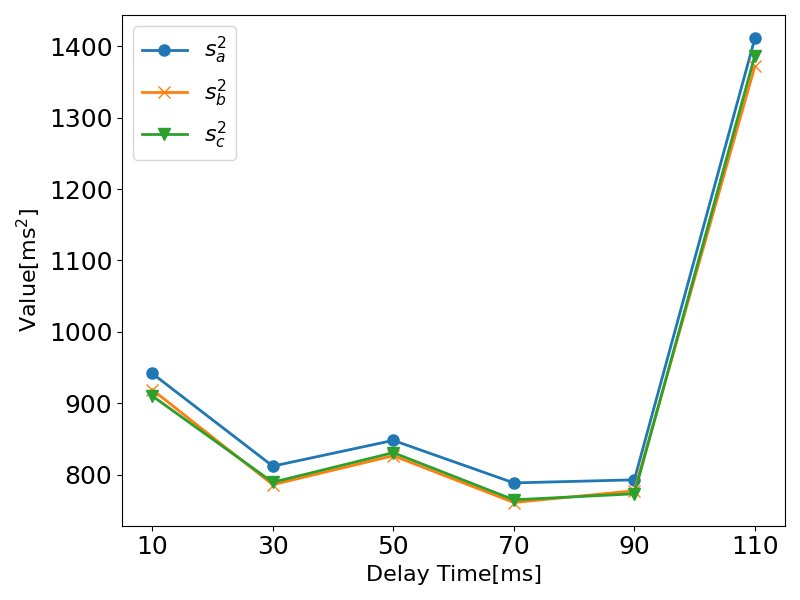
\includegraphics[scale=0.5]{figures/Yobi/Var/Normal_bunnsann.png}
  \caption{遅延時間と評価指標の関係}
  \label{fig:Normal_bunsan}
\end{figure}
\begin{figure}[bt]
  \centering
  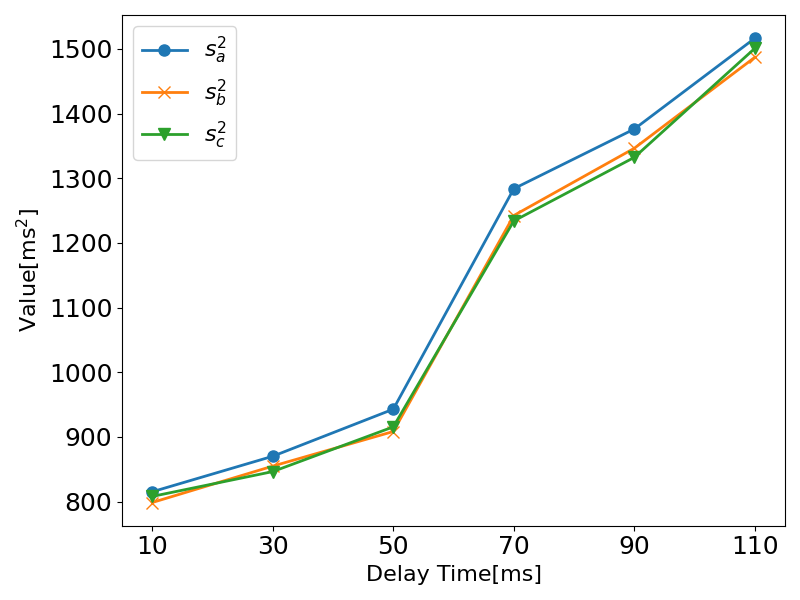
\includegraphics[scale=0.5]{figures/Yobi/Var/Unique_bunsan.png}
  \caption{遅延時間と評価指標の関係}
  \label{fig:Unique_bunsan}
\end{figure}
\begin{figure}[bt]
  \centering
  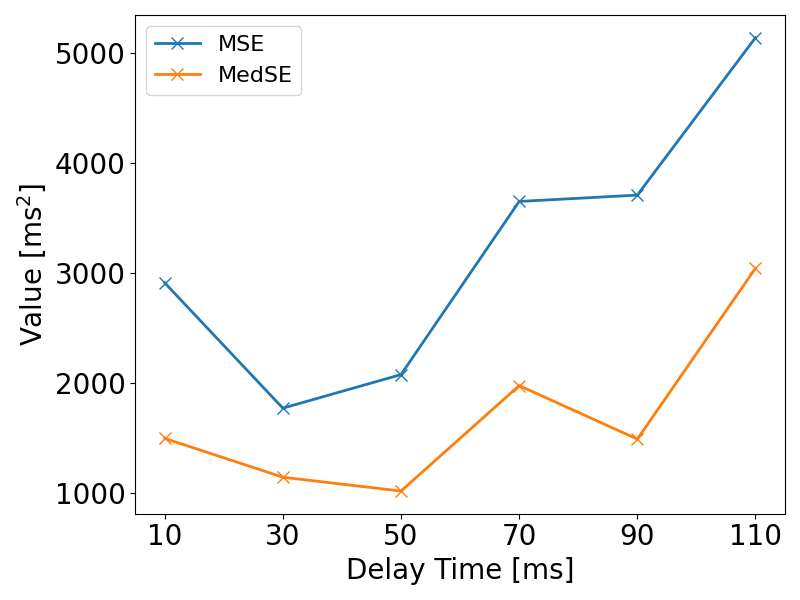
\includegraphics[scale=0.5]{figures/Yobi/Var/MSE_MedSE.png}
  \caption{遅延時間とMSEおよびMedSEの関係}
  \label{fig:Yobi_MSE_MedSE}
\end{figure}
図\ref{fig:Normal_bunsan}における実験Aによる遅延聴覚フィードバックの身体運動への影響の調査結果と,図\ref{fig:Unique_bunsan}における提示順1による同様の影響調査結果を提示する.図\ref{fig:Normal_bunsan}に示される結果から,10[ms]から70[ms]の間で評価指標が減少傾向を示し,90[ms]から110[ms]の範囲では評価指標が急激に増加していることが観察される.
30[ms]から90[ms]の間で評価指標が減少した原因としては,被験者の馴化が挙げられる.合図音の遅延が一貫しているシステム設計においては,ボタン押し課題の繰り返しにより,被験者は課題に慣れ,大きな遅延にも順応してしまうことが示唆される.
対照的に,図\ref{fig:Unique_bunsan}では,10[ms]の評価値が最小であり,遅延時間の増加に伴い評価値が上昇する傾向が見られる.これは,4回に1回の遅延が身体運動に与える影響を示唆する結果である.したがって,本研究では「ボタン押下時の合図音の遅延が一定であれば,被験者は遅延に馴染み,ボタン押下時間間隔に及ぼす影響が減少する」という仮説を支持し,次回以降の実験では,実験Bの条件下での調査を実施することとする.

% コメントアウト
% \begin{figure}[bt]
%   \centering
%   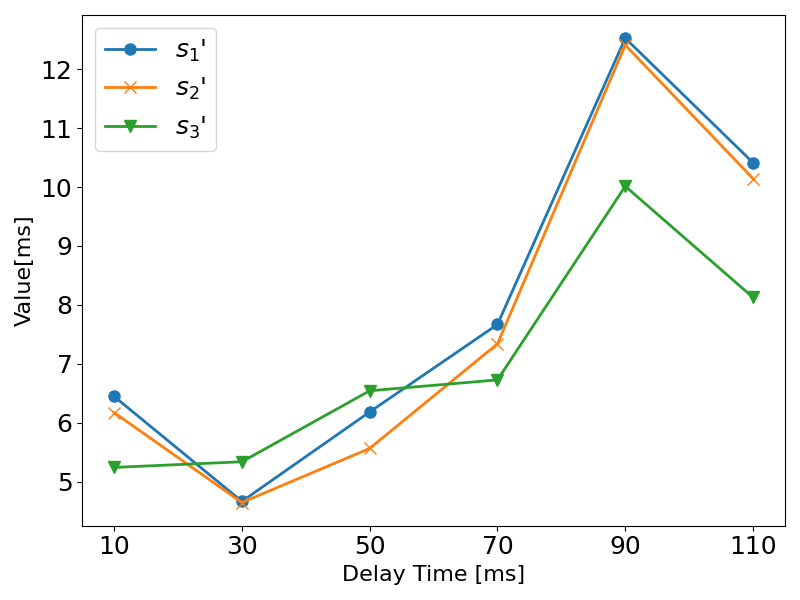
\includegraphics[scale=0.5]{figures/Yobi/Yobi_2And2_110ms.png}
%   \caption{直前と直後2回ずつ}
% \end{figure}
\newpage \newpage
% \section{遅延への順応の示唆}
% 文献[重松さんの修論]では,分析するデータの開始点によって,評価値の値が変化すると報告されている.そこで,本節でも,6.3節の結果から示唆された遅延への順応について,分析対象のデータの開始点を様々に変化させることによって,遅延への順応の可能性を検証し,今後の調査に役立てる.
